\documentclass[letterpaper,12pt]{article}

\usepackage[utf8]{inputenc} % Soporte para acentos
\usepackage[T1]{fontenc}    
\usepackage[spanish,mexico]{babel} % Español

% Soporte de símbolos adicionales (matemáticas)
\usepackage{amsmath}		
\usepackage{amssymb}		
\usepackage{amsfonts}
\usepackage{latexsym}

% Para inserción de imagenes
\usepackage[pdftex]{graphicx}

\usepackage[lmargin=2cm,rmargin=2cm,top=2cm,bottom=2cm]{geometry}

% Información para el título
\title{Imagenes}
\author{J. Luis Torres}

\begin{document}

\maketitle

Ejemplos de figuras insertadas en un documento de \LaTeX{}.

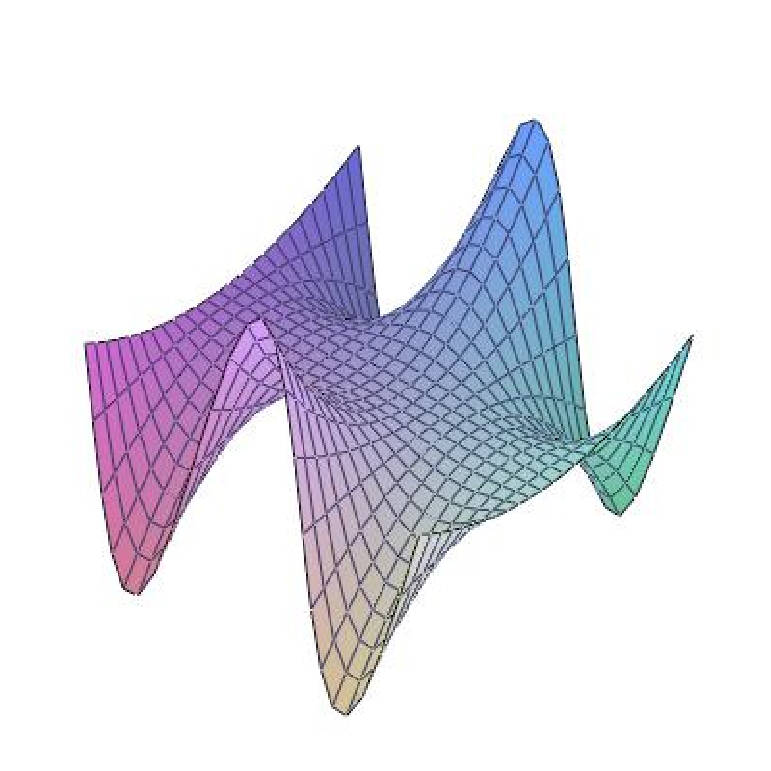
\includegraphics{grafica10.jpg}

\newpage

\begin{figure}[h!]
\centering
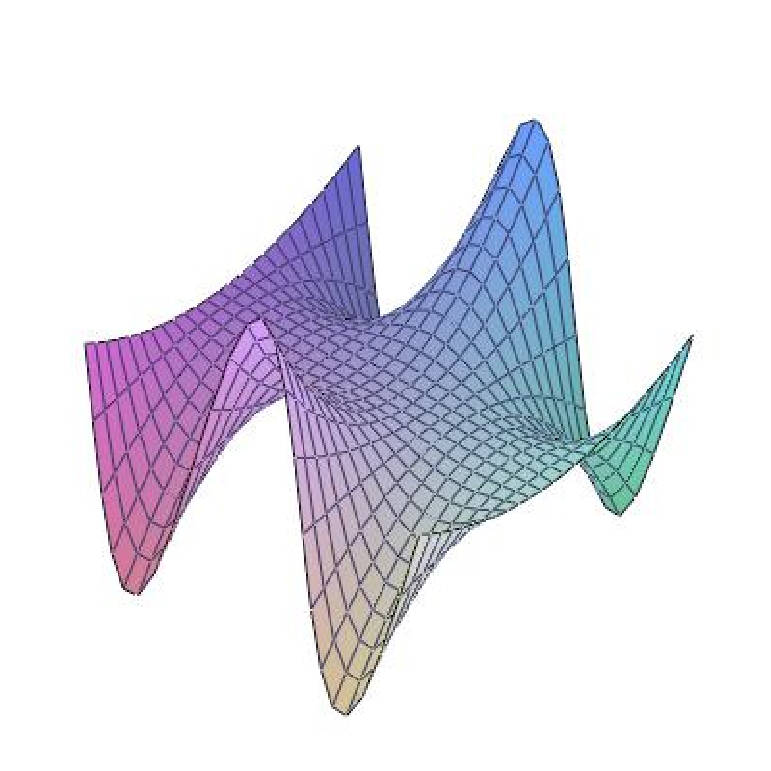
\includegraphics[scale=0.5]{grafica10.jpg}
\caption{Gráfica de $x^2 \cdot \cos (y)$}
\end{figure}

\end{document}
